\chapter{Sprint 01 : Implémentation du module Gestion des clients}

\section*{Introduction}

Dans le cadre de la démarche agile adoptée pour ce projet, le premier sprint a été consacré à l’implémentation du module de \textbf{gestion des clients}. Ce module constitue une brique essentielle du système, car il permet l’enregistrement, l’administration et l’exploitation des informations relatives aux utilisateurs finaux (clients particuliers ou professionnels).

L’objectif principal de ce sprint était de concevoir une structure de données robuste, de développer une interface utilisateur intuitive, et d’assurer la communication fluide entre le frontend Angular et le backend Django via des appels API REST sécurisés.

Ce chapitre présente :
\begin{itemize}
    \item Le backlog associé au Sprint 01,
    \item Le diagramme de cas d’utilisation spécifique à ce module,
    \item Les entités et modèles de données implémentés,
    \item L’interface utilisateur (Angular),
    \item Les endpoints API côté backend (Django),
    \item Et enfin, les contraintes rencontrées et les choix techniques réalisés.
\end{itemize}

\section{Sprint 01 Backlog}
\begin{table}[H]
\centering

\begin{tabular}{|c|p{3.8cm}|c|p{4.5cm}|c|c|}
\hline
\textbf{ID US} & \textbf{User Story} & \textbf{ID Task} & \textbf{Task} & \textbf{Estimation} & \textbf{Responsable} \\
\hline

US01 & En tant que client, je peux créer un compte avec mes informations personnelles.
     & US01.1 & Créer le modèle Client (Django) & 2h & Aziz \\
     \cline{3-6}
     & & US01.2 & Développer l’API d’inscription & 2h & Aziz \\
     \cline{3-6}
     & & US01.3 & Créer le formulaire Angular & 2h & Aziz \\
\hline

US02 & En tant que client, je peux gérer mon profil utilisateur. 
     & US02.1 & Développer l’API de modification de profil & 2h & Aziz \\
     \cline{3-6}
     & & US02.2 & Créer l’interface de gestion de profil & 2h & Aziz \\
\hline

US03 & En tant que client, je peux soumettre une demande via un chatbot.
     & US03.1 & Implémenter la logique du chatbot & 3h & Aziz \\
     \cline{3-6}
     & & US03.2 & Relier le chatbot au backend (création d’ordre) & 2h & Aziz \\
\hline

US04 & En tant que client, je peux consulter mes demandes passées.
     & US04.1 & Créer le composant Angular d’historique des demandes & 2h & Aziz \\
     \cline{3-6}
     & & US04.2 & Implémenter l’API de récupération des ordres client & 2h & Aziz \\
\hline

US05 & En tant que client, je peux voir les prestataires intéressés.
     & US05.1 & Développer l’API de récupération des intéressés & 2h & Aziz \\
     \cline{3-6}
     & & US05.2 & Afficher les profils dans l’interface de l’ordre & 1h & Aziz \\
\hline

US06 & En tant que client, je peux discuter avec le prestataire.
     & US06.1 & Intégrer une messagerie client-prestataire & 3h & Aziz \\
\hline

US07 & En tant que client, je reçois une facture après la mission.
     & US07.1 & Générer automatiquement la facture (backend) & 2h & Aziz \\
     \cline{3-6}
     & & US07.2 & Envoyer la facture par e-mail & 1h & Aziz \\
\hline

\end{tabular}
\caption{Product Backlog – Module Gestion des clients}
\label{tab:product_backlog_clients}
\end{table}

\section{Diagramme de cas d'utilisation raffiné}

Le diagramme suivant représente une vue raffinée des interactions possibles entre un \textbf{Client} et le système. Il met en évidence les cas d’utilisation principaux ainsi que les relations de type \textit{<<include>>} et \textit{<<extend>>}, permettant une meilleure modélisation des comportements facultatifs et réutilisables.

\begin{figure}[H]
    \centering
    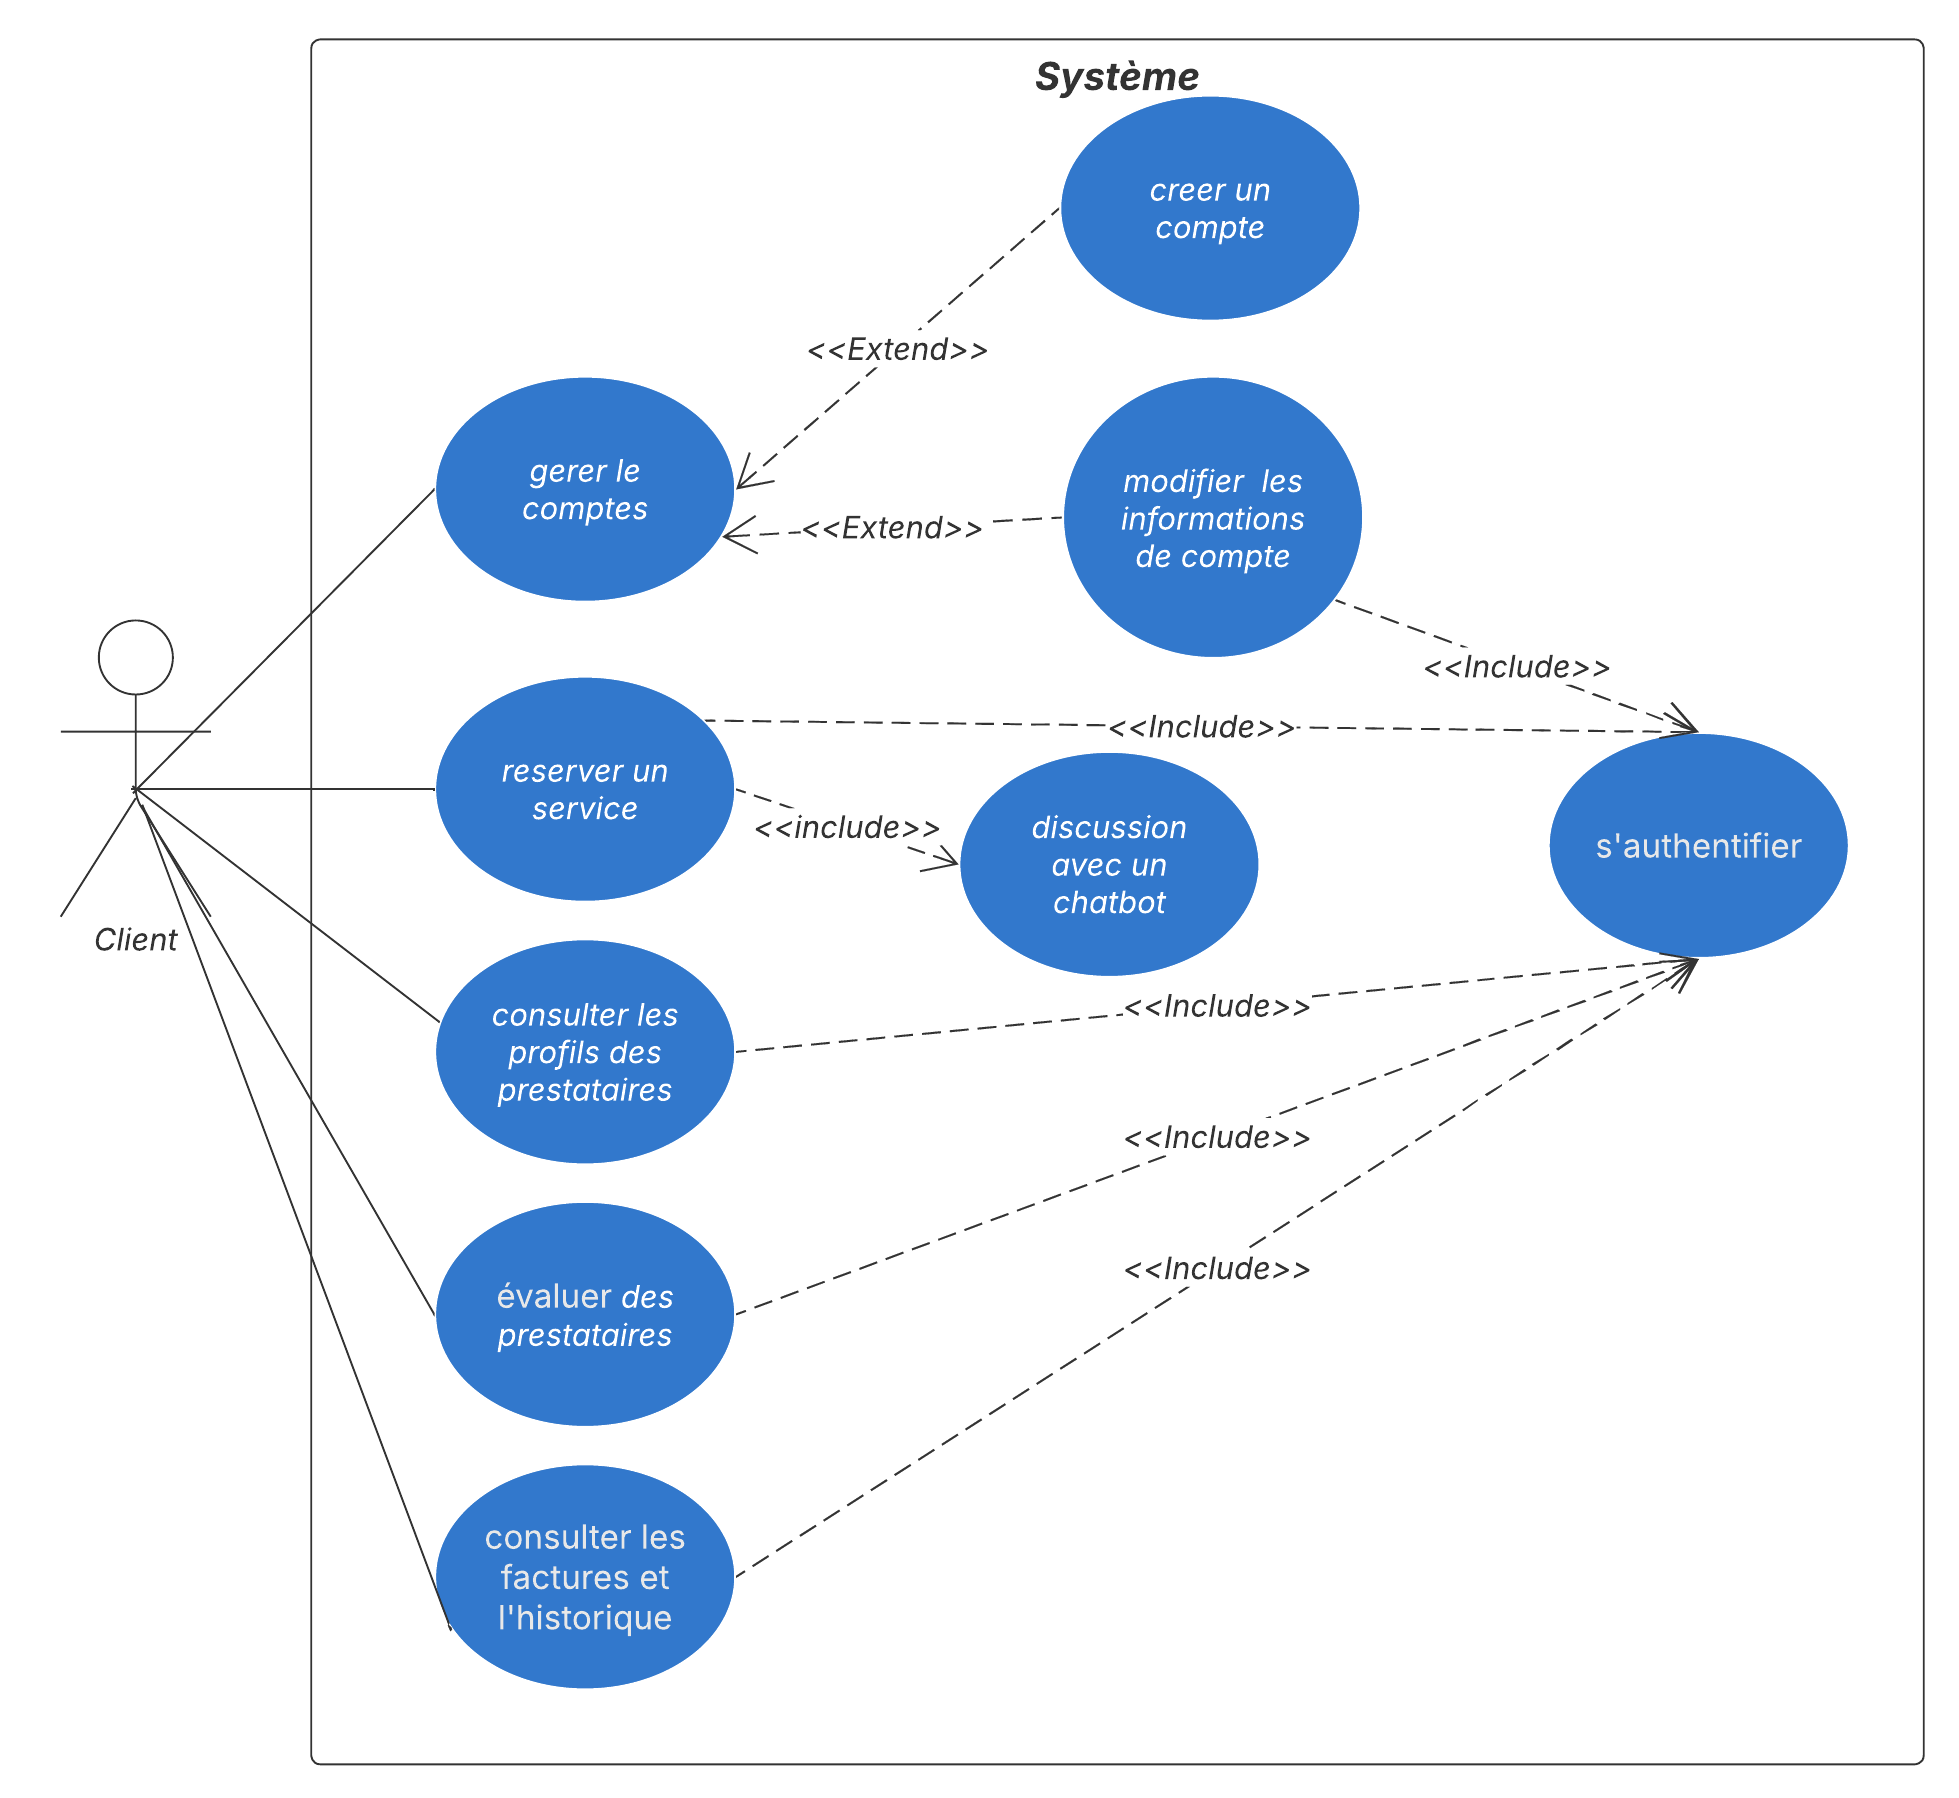
\includegraphics[width=0.9\textwidth]{figures/Diagramme de cas d'utilisation.png}
    \caption{Diagramme de cas d'utilisation raffiné – Gestion des clients}
    \label{fig:usecase_raffine_client}
\end{figure}

\noindent
Ce diagramme montre que le \textbf{Client} peut :
\begin{itemize}
    \item \textbf{Gérer son compte}, avec extension possible vers la création ou la modification des informations personnelles.
    \item \textbf{Réserver un service}, incluant une interaction préalable avec un chatbot.
    \item \textbf{Consulter les profils des prestataires}, ainsi que leurs évaluations.
    \item \textbf{Consulter l’historique des commandes et les factures associées}.
\end{itemize}

Toutes ces fonctionnalités reposent sur une action préalable indispensable : \textbf{s’authentifier}, indiquée par les relations de type \textit{<<include>>}. Cette modélisation renforce la clarté des scénarios d’utilisation et leur dépendance aux conditions d’accès.

\section{Diagrammes de séquence}
Le \textbf{diagramme de séquence UML} est un diagramme comportemental utilisé pour modéliser les interactions dynamiques entre les différents acteurs (utilisateurs ou systèmes) et les composants du système au fil du temps. Il décrit l'enchaînement chronologique des messages échangés entre les entités dans un scénario précis.

Ce diagramme met en évidence :
\begin{itemize}
    \item les acteurs ou composants impliqués (ex : Client, Interface Angular, Backend Django, Base de données) ;
    \item les messages transmis (requêtes, réponses, appels de fonction) ;
    \item l’ordre d’exécution des actions.
\end{itemize}

Il est particulièrement utile pour visualiser le déroulement d’un cas d’utilisation, vérifier la cohérence des appels API et anticiper la logique métier lors de l’implémentation technique.
\subsection*{Création de compte client}
\begin{figure}[H]
\centering
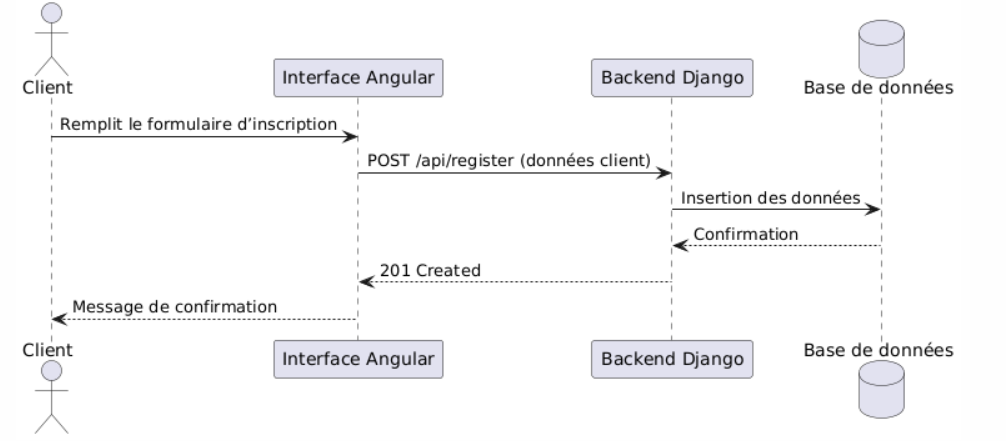
\includegraphics[width=0.85\linewidth]{figures/Séquence – Création de compte client.png}
\caption{Diagramme de séquence – Création d’un compte client}
\end{figure}
\textit{Ce diagramme décrit le processus d’enregistrement d’un nouveau client. Le client saisit ses informations dans un formulaire Angular. Une requête POST est ensuite envoyée au backend Django via un endpoint REST /api/register. Le backend se charge de l’insertion des données dans la base PostgreSQL, puis renvoie une confirmation de succès. Enfin, l’interface affiche un message confirmant la création du compte. Ce scénario met en évidence l’intégration fluide entre le frontend et le backend dans une architecture orientée services.}

\vspace{1em}

\subsection*{Soumission d’une demande via le chatbot}
\begin{figure}[H]
\centering
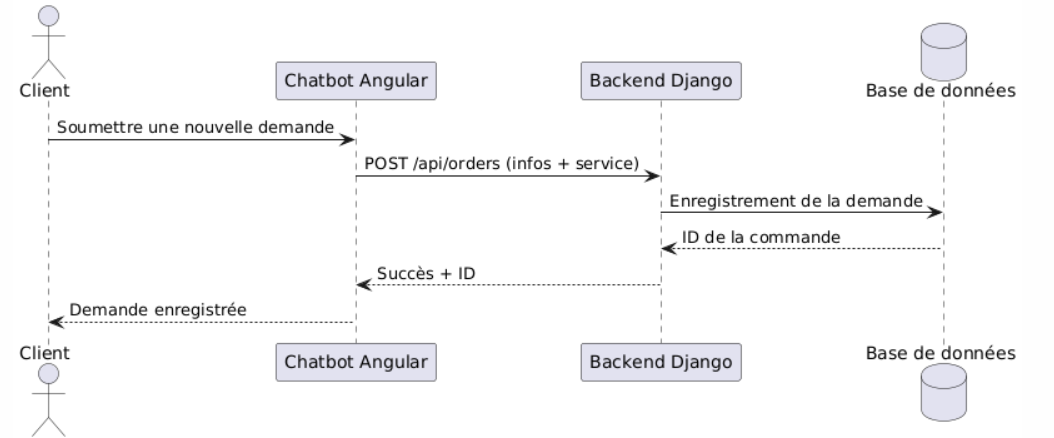
\includegraphics[width=0.90\linewidth]{figures/Séquence – Soumettre une demande via le chatbot.png}
\caption{Diagramme de séquence – Soumission d’une demande via le chatbot}
\end{figure}
\textit{Ce diagramme illustre comment un client initie une demande de prestation à travers le chatbot intégré à l’interface Angular. Une fois les informations collectées (type de service, description, coordonnées), une requête POST est envoyée au backend Django sur l’endpoint /api/orders. Après validation et enregistrement, le backend retourne un identifiant unique de la commande. Le client reçoit une confirmation que sa demande a bien été enregistrée. Cette interaction favorise une expérience utilisateur rapide et automatisée.}

\vspace{1em}

\subsection*{Modification du profil client}
\begin{figure}[H]
\centering
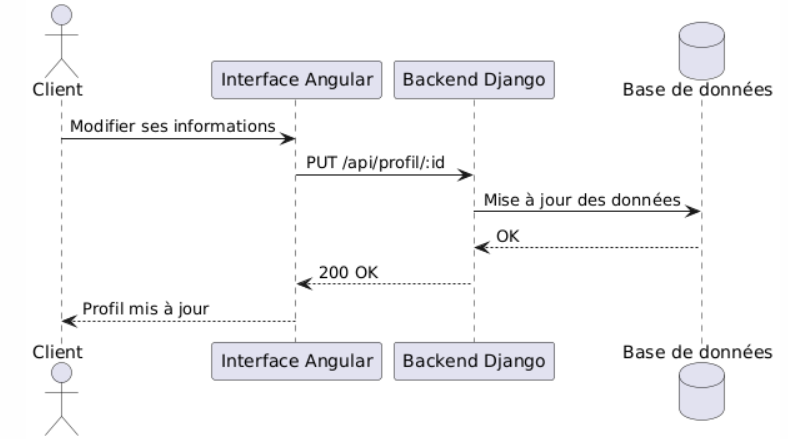
\includegraphics[width=0.85\linewidth]{figures/Séquence – Modification du profil client.png}
\caption{Diagramme de séquence – Mise à jour du profil client}
\end{figure}
\textit{Ce diagramme retrace le scénario dans lequel un client modifie ses informations personnelles. Les données modifiées sont envoyées via une requête PUT sur l’endpoint /api/profil/:id. Le backend Django traite la requête, met à jour les informations dans la base, puis retourne une réponse HTTP 200 OK. L’interface informe ensuite le client que les modifications ont été prises en compte. Ce flux garantit la cohérence des données utilisateurs.}

\section{Diagrammes d’activité}
Le \textbf{diagramme d’activité UML} est un diagramme comportemental permettant de représenter les différentes étapes d’un processus métier sous forme de flux d’activités. Il est souvent utilisé pour modéliser les workflows, les logiques conditionnelles et les prises de décision.

Il permet de :
\begin{itemize}
    \item illustrer l’enchaînement logique des actions d’un utilisateur ou d’un système ;
    \item intégrer des conditions, des boucles ou des actions parallèles ;
    \item clarifier la logique métier avant le développement technique.
\end{itemize}

\subsection*{Création de compte client}
\begin{figure}[H]
\centering
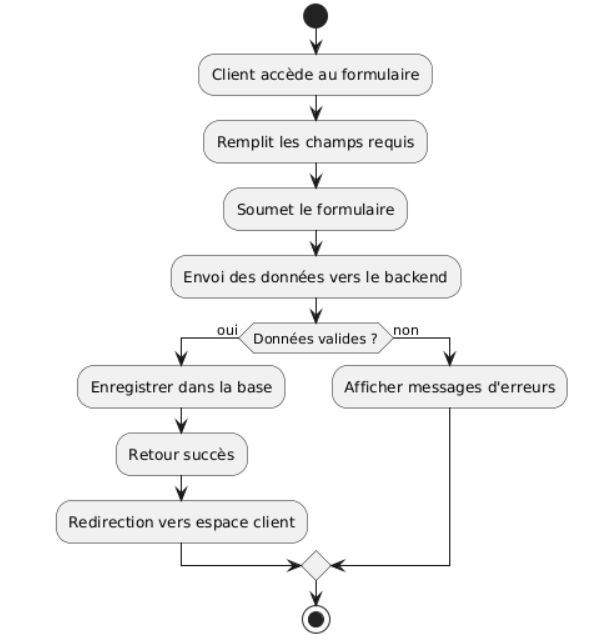
\includegraphics[width=0.60\linewidth]{figures/Activité – Création de compte client.png}
\caption{Diagramme d’activité – Création de compte client}
\end{figure}
\textit{Ce diagramme montre les étapes fonctionnelles du processus de création de compte. Après avoir accédé au formulaire, le client saisit ses informations, puis soumet le formulaire. Le backend valide les données reçues. Si les champs sont valides, les données sont enregistrées ; dans le cas contraire, des messages d’erreur sont affichés. Ce diagramme met en évidence les flux de validation côté serveur et les interactions conditionnelles.}

\vspace{1em}

\subsection*{Consultation de ses demandes}
\begin{figure}[H]
\centering
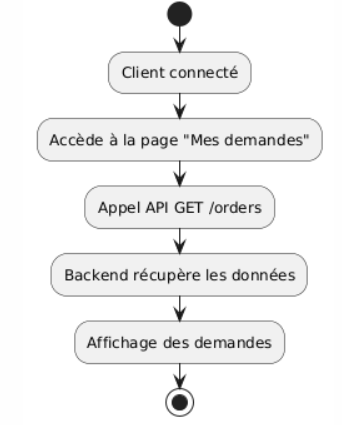
\includegraphics[width=0.55\linewidth]{figures/Activité – Consultation de ses demandes.png}
\caption{Diagramme d’activité – Consultation des demandes passées}
\end{figure}
\textit{Le diagramme décrit la logique de consultation des demandes effectuées par un client connecté. Une fois connecté, celui-ci accède à la page “Mes demandes”. Un appel API de type GET est déclenché vers le backend qui récupère les données depuis la base et les renvoie pour affichage. Ce processus montre un accès simple et direct à l’historique utilisateur.}

\vspace{1em}

\subsection*{Messagerie avec un prestataire}
\begin{figure}[H]
\centering
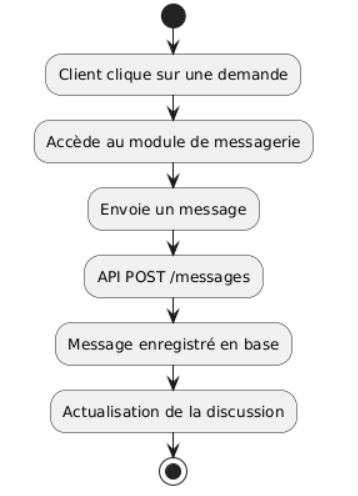
\includegraphics[width=0.55\linewidth]{figures/Activité – Messagerie avec prestataire.png}
\caption{Diagramme d’activité – Messagerie client-prestataire}
\end{figure}
\textit{Ce diagramme d’activité présente l’enchaînement des actions lors de l’envoi d’un message par le client. Une fois sur une demande spécifique, le client accède au module de messagerie. Le message rédigé est envoyé via une requête POST vers /messages. Après enregistrement en base, la discussion est actualisée. Ce diagramme reflète le caractère temps réel de la communication au sein de la plateforme.}
\section{Interfaces utilisateur Angular}

Cette section présente les différentes interfaces développées avec Angular pour les utilisateurs de la plateforme Swift Helpers. Chaque capture d’écran est accompagnée d’un commentaire expliquant son objectif fonctionnel.

\begin{figure}[H]
    \centering
    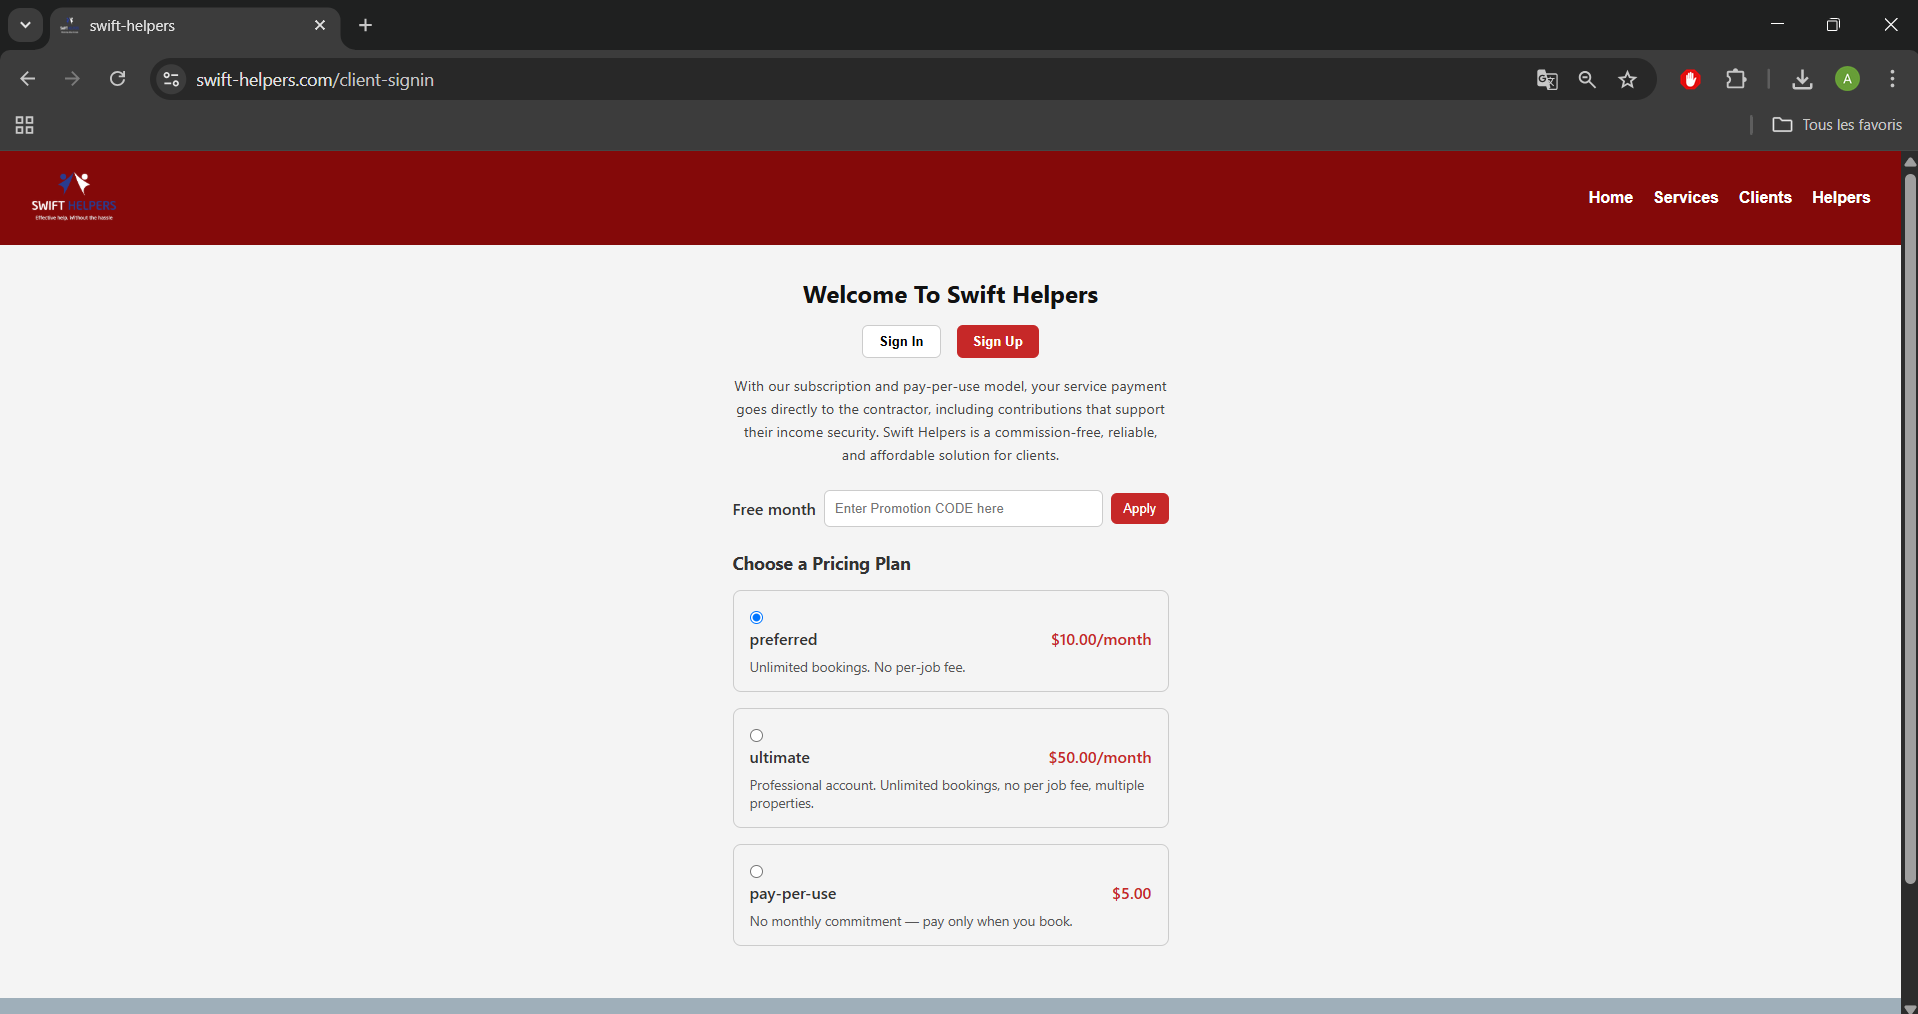
\includegraphics[width=0.95\textwidth]{figures/gestion de compte client.png}
    \caption{Page d'inscription client avec choix du plan d'abonnement}
\end{figure}

\noindent
Cette interface permet aux clients de s’inscrire à la plateforme en choisissant un plan tarifaire (preferred, ultimate ou pay-per-use). Elle joue un rôle essentiel dans la gestion des accès selon les privilèges associés à chaque abonnement.

\vspace{0.5cm}

\begin{figure}[H]
    \centering
    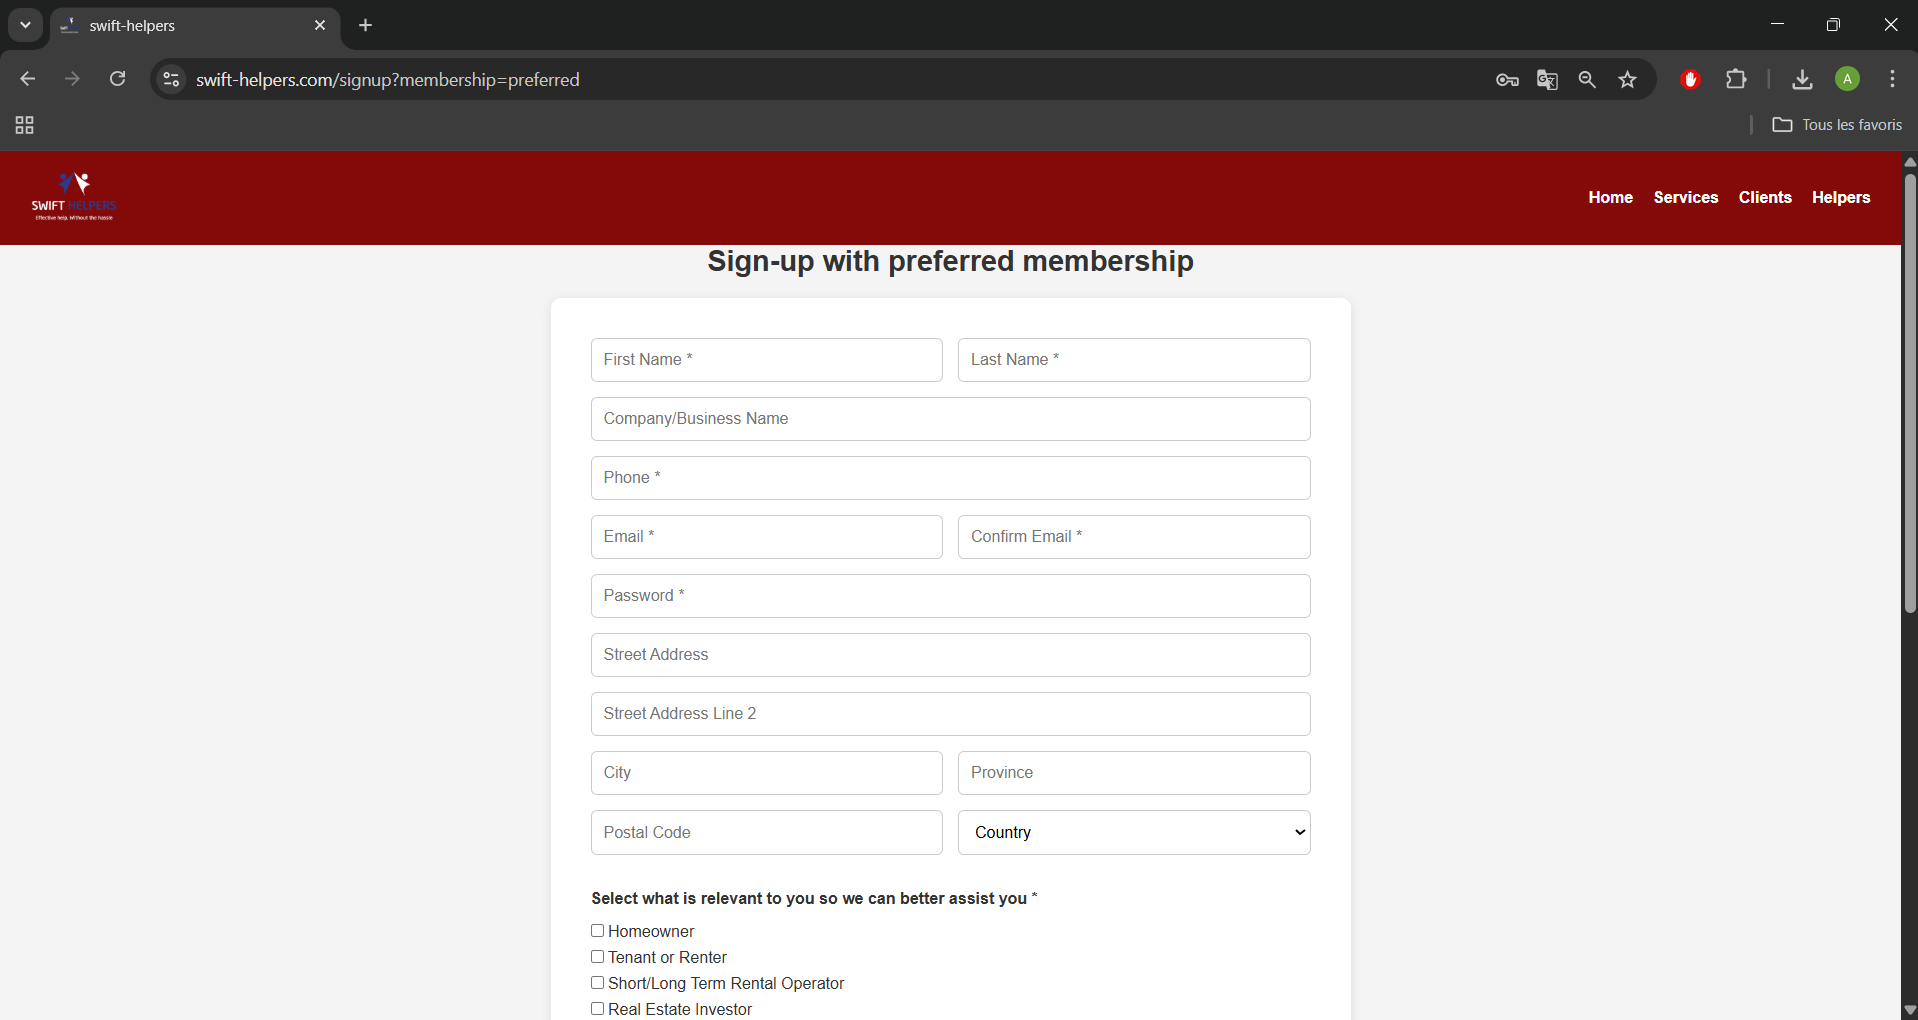
\includegraphics[width=0.95\textwidth]{figures/inscription client.png}
    \caption{Formulaire d’inscription détaillée du client}
\end{figure}

\noindent
Cette vue affiche le formulaire d’inscription, avec collecte des informations personnelles, professionnelles et de contact. Le formulaire est dynamique, conditionné par le type d’utilisateur ou le plan choisi.


\vspace{0.5cm}

\begin{figure}[H]
    \centering
    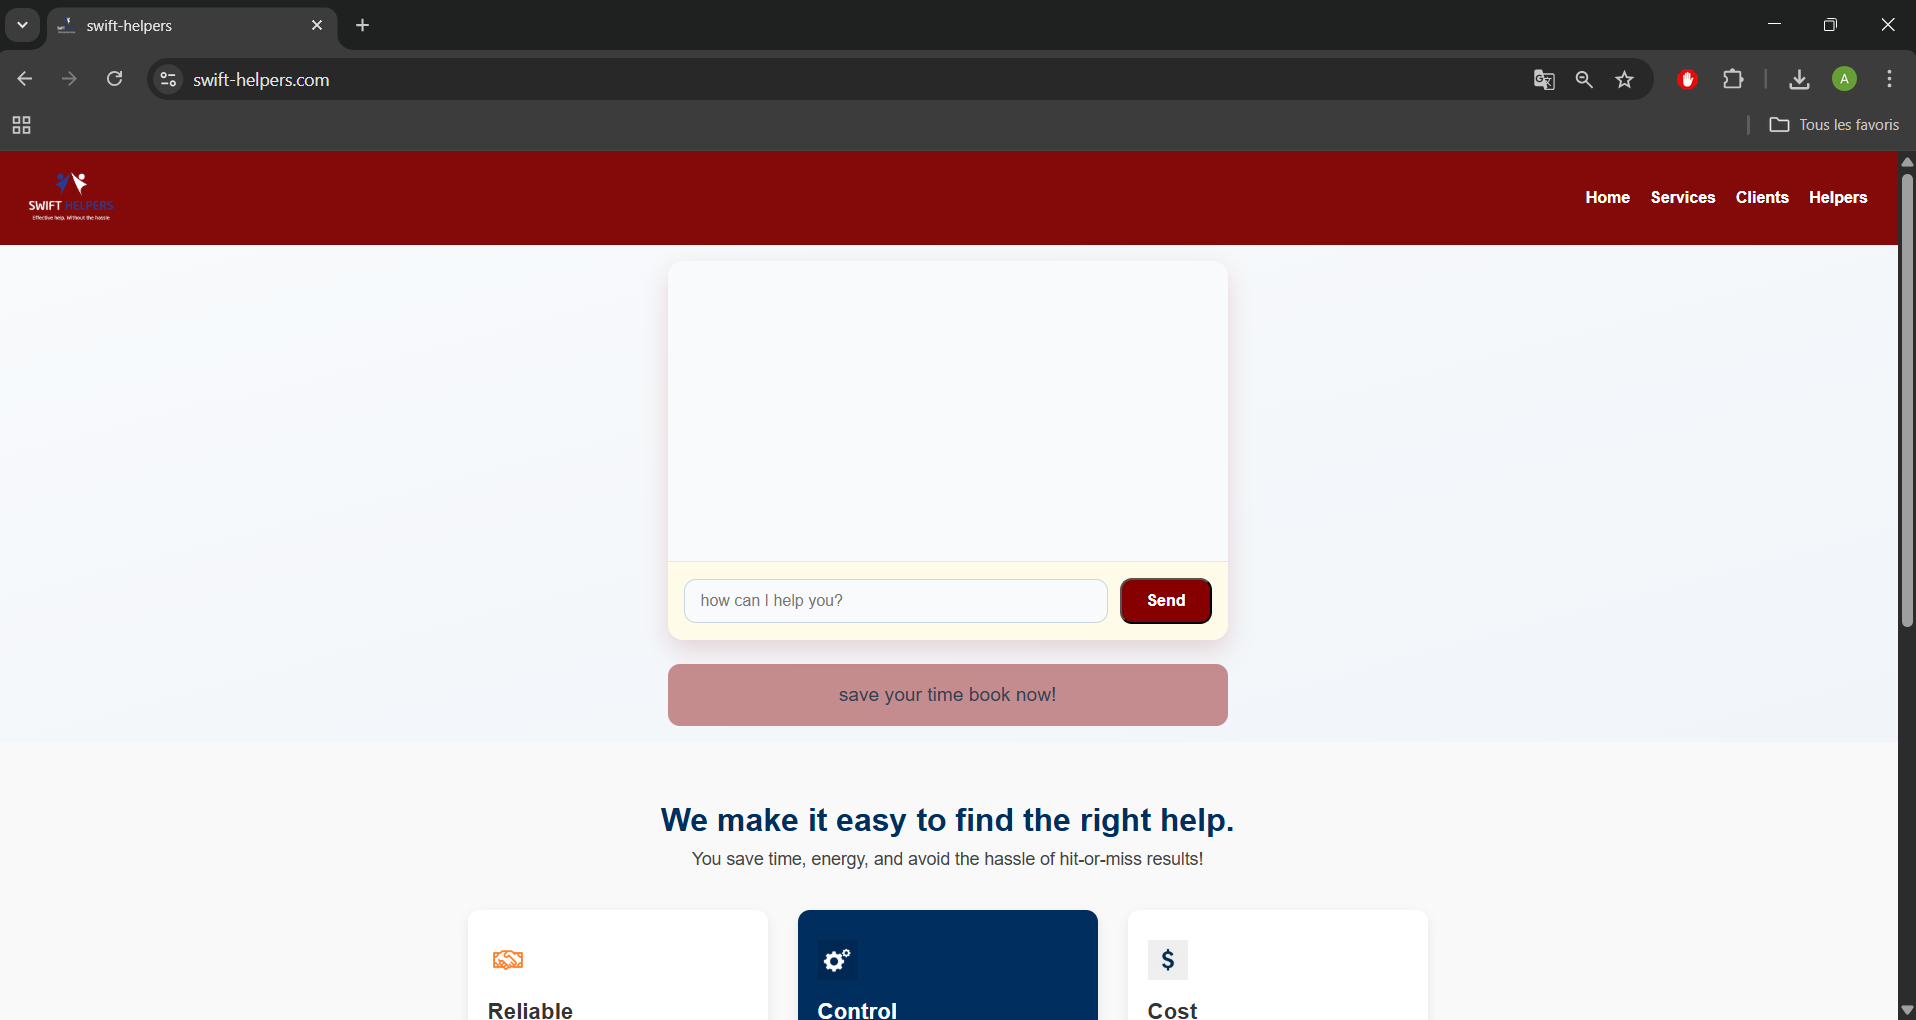
\includegraphics[width=0.85\textwidth]{figures/interface principale.png}
    \caption{Interface du chatbot conversationnel}
\end{figure}

\noindent
Cette interface permet une interaction directe entre le client et un agent conversationnel. Le chatbot guide le client dans la soumission d’une demande de service de manière naturelle et fluide.

\vspace{0.5cm}

\begin{figure}[H]
    \centering
    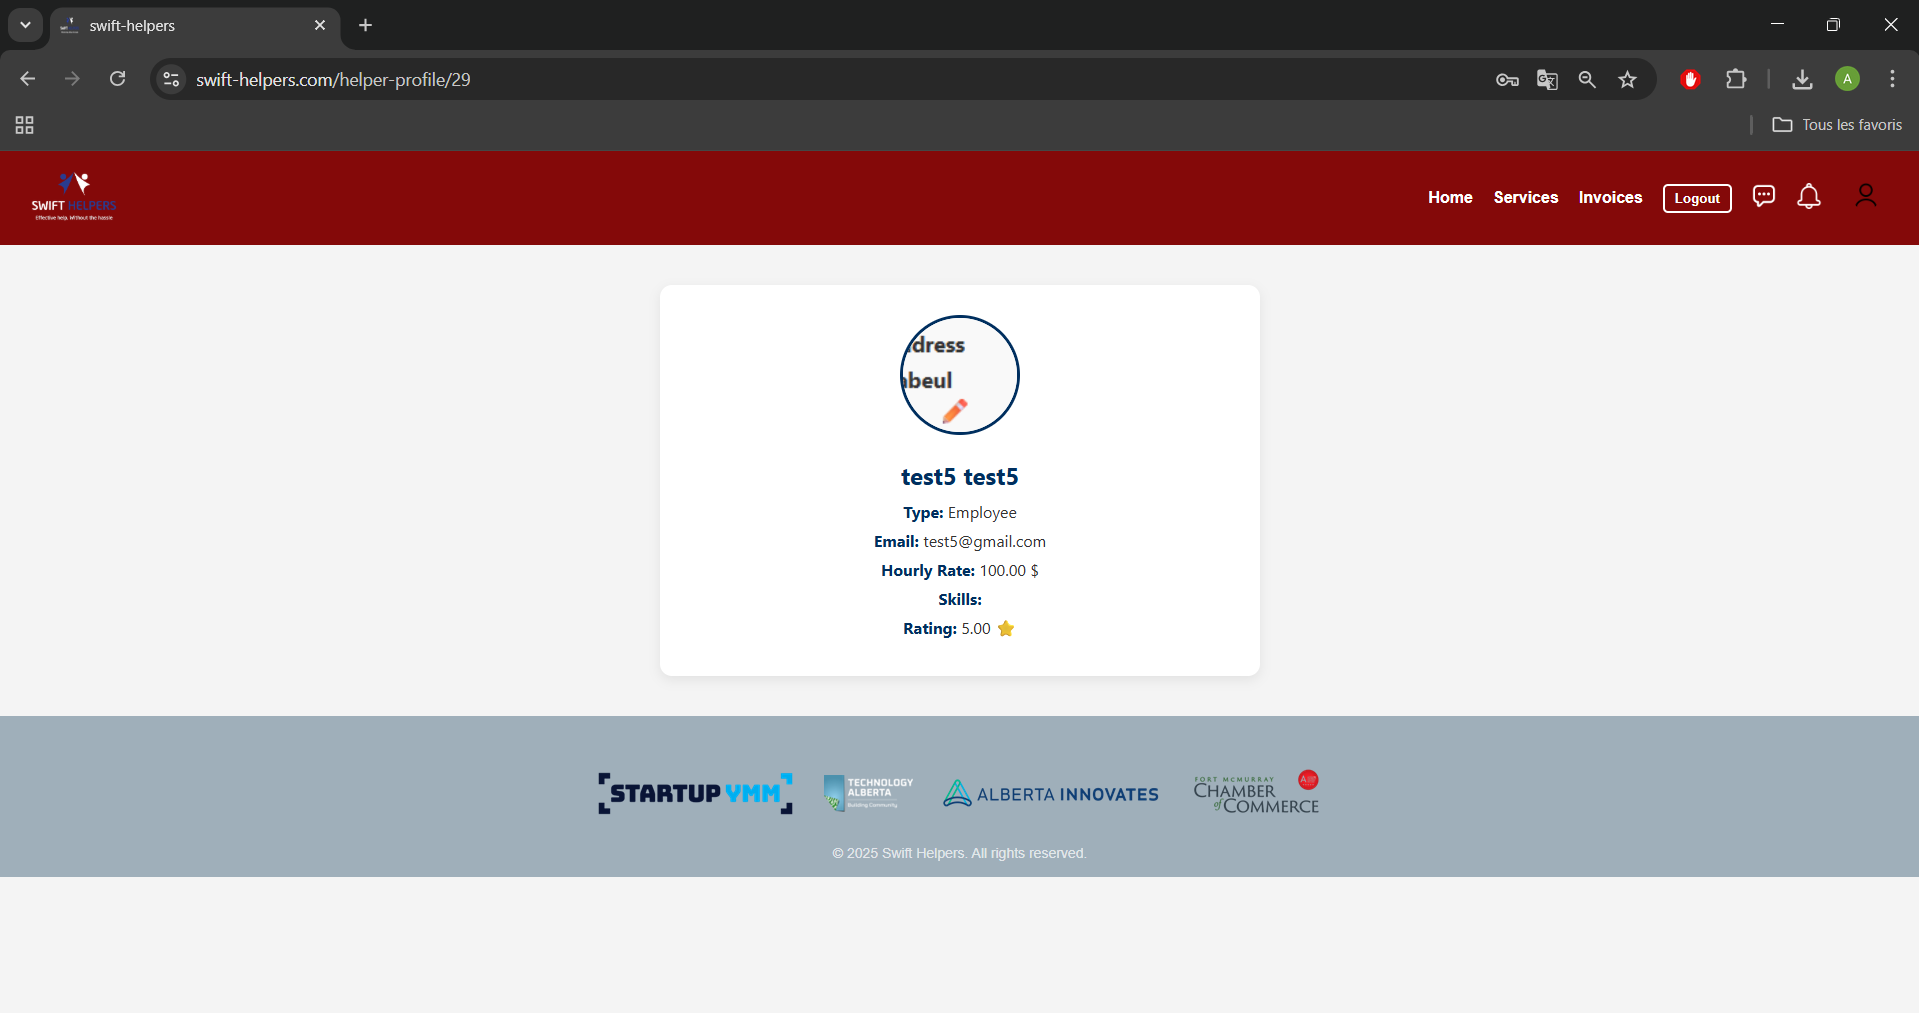
\includegraphics[width=0.9\textwidth]{figures/profil helper.png}
    \caption{Profil détaillé d’un helper (prestataire)}
\end{figure}

\noindent
Cette interface affiche le profil public d’un prestataire avec son tarif horaire, ses compétences et sa notation. Elle est consultable par le client au moment de choisir un intervenant.

\vspace{0.5cm}

\begin{figure}[H]
    \centering
    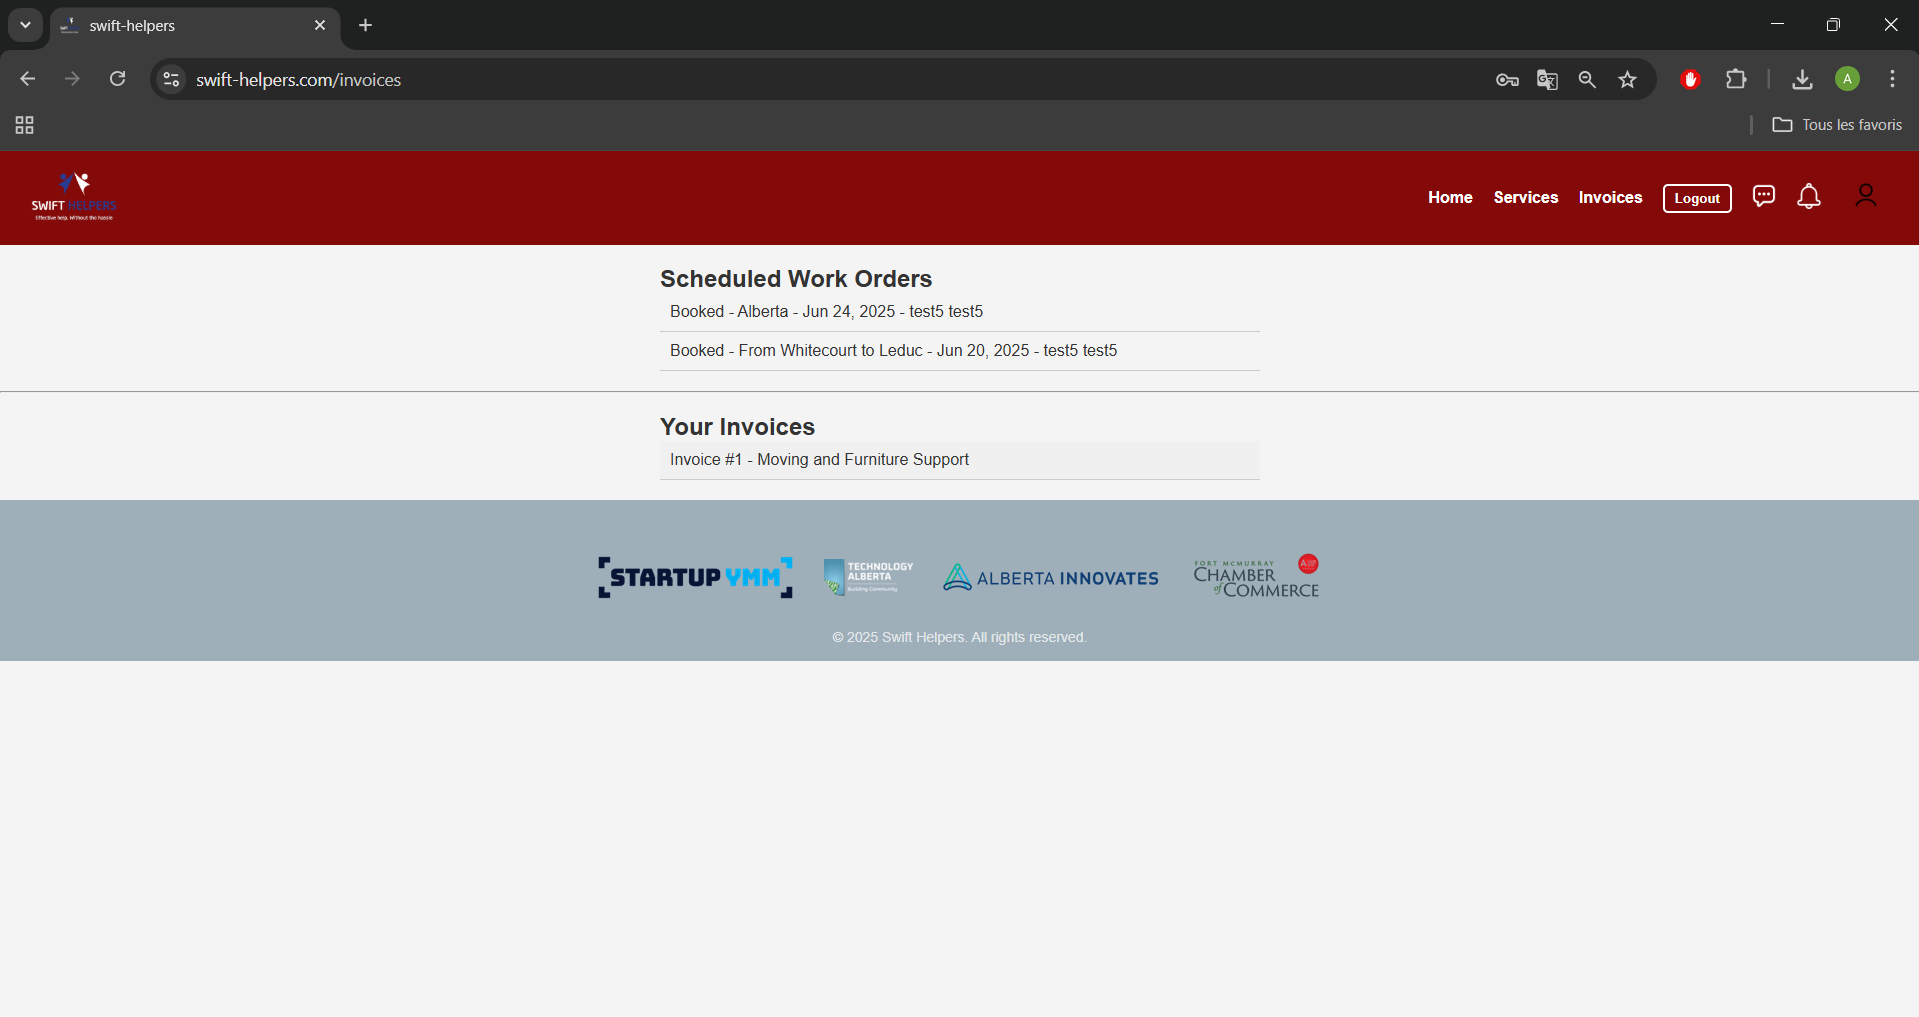
\includegraphics[width=0.9\textwidth]{figures/facture client.png}
    \caption{Liste des commandes et des factures associées}
\end{figure}

\noindent
Cette page permet au client de consulter l’historique de ses demandes de services, ainsi que les factures associées. Elle favorise la transparence et la traçabilité des interventions.

\section{Aperçue Sur Le Code}

Cette section présente des extraits significatifs du code source de l'application, développée avec le framework Angular (frontend) et Django (backend). Chaque capture illustre un fichier clé ou une fonctionnalité technique centrale.

\begin{figure}[H]
    \centering
    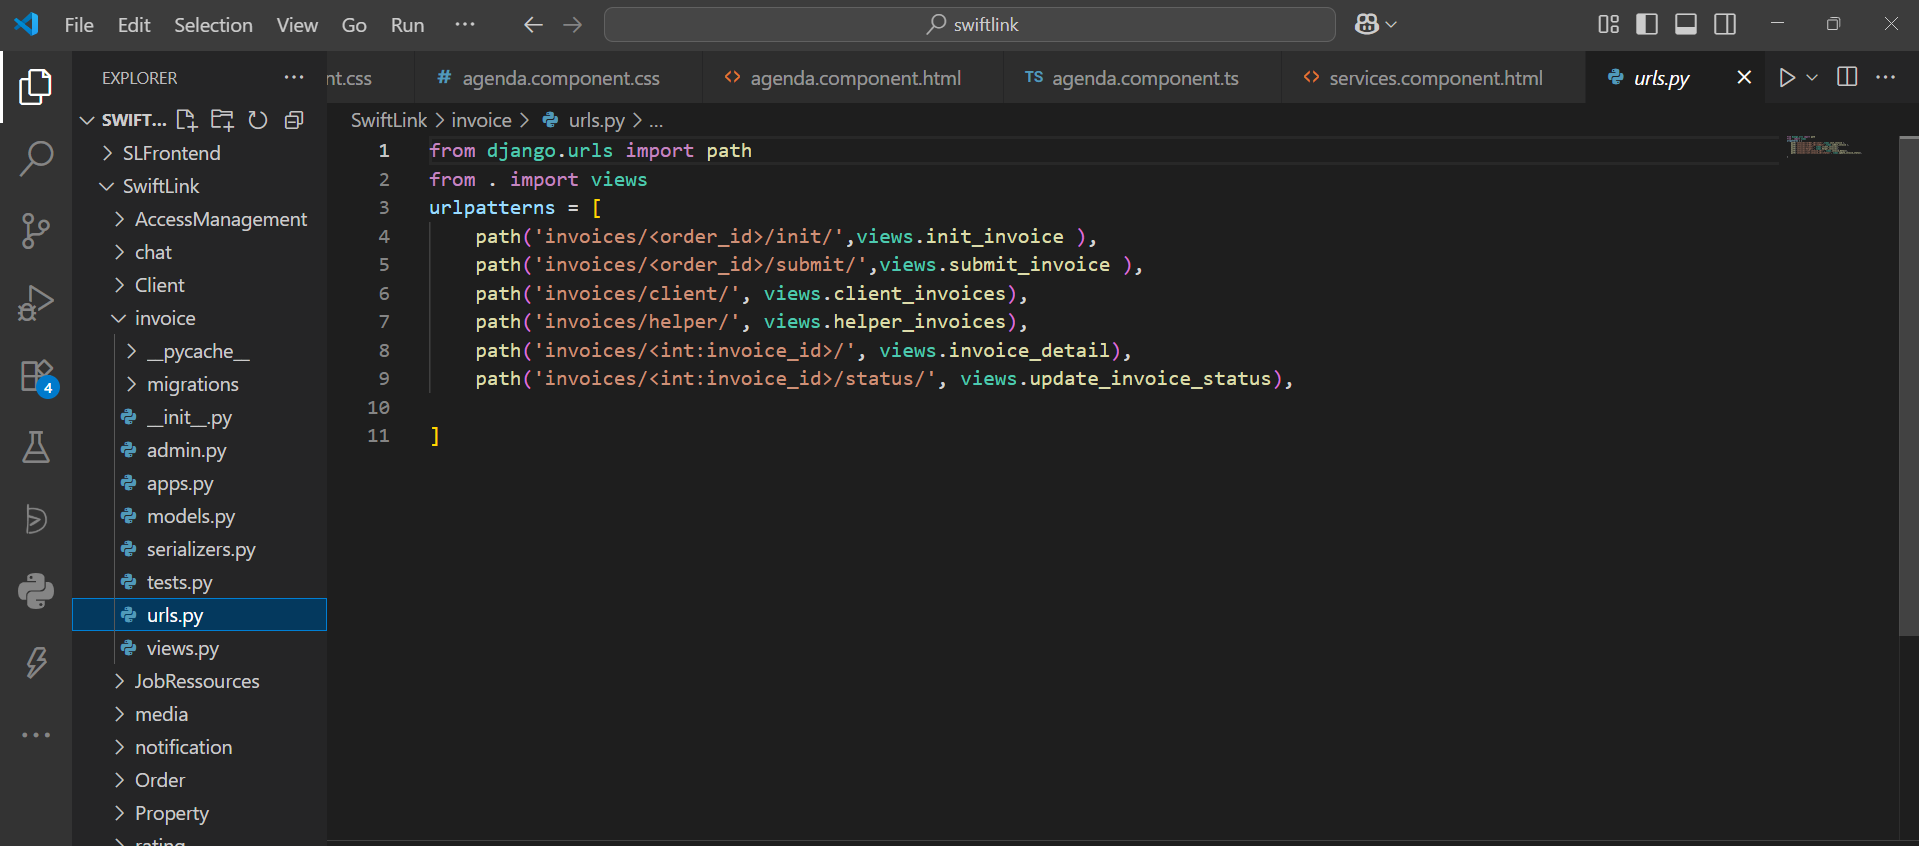
\includegraphics[width=0.9\textwidth]{figures/urls.png}
    \caption{Déclaration des routes d'API – Module Invoice (Django)}
\end{figure}

\noindent
Ce fichier \texttt{urls.py} configure les routes REST associées à la gestion des factures. On y retrouve notamment :
\begin{itemize}
    \item L'initialisation et la soumission d'une facture pour une commande spécifique.
    \item La récupération des factures côté client ou helper.
    \item Le détail d'une facture et la mise à jour de son statut.
\end{itemize}

\vspace{0.5cm}

\begin{figure}[H]
    \centering
    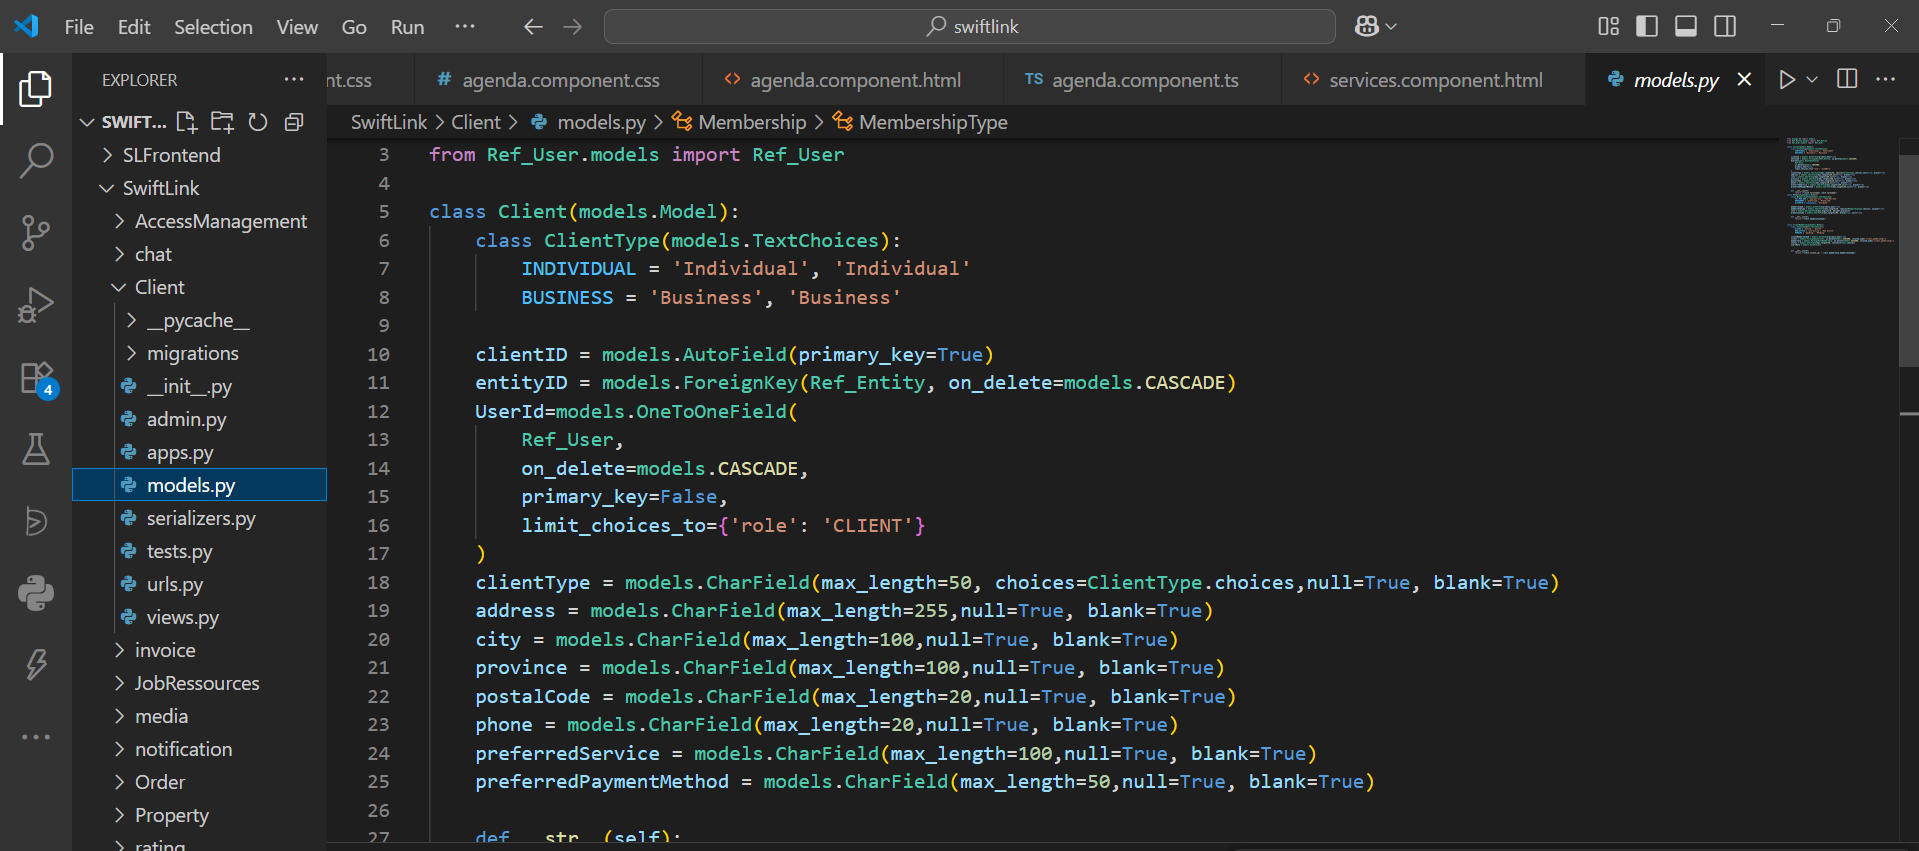
\includegraphics[width=0.95\textwidth]{figures/modele client.png}
    \caption{Modèle Django – Client (models.py)}
\end{figure}

\noindent
Le modèle \texttt{Client} décrit la structure des données associées à un utilisateur client. Il contient des champs relatifs à :
\begin{itemize}
    \item Ses coordonnées et préférences.
    \item Son rattachement à une entité organisationnelle.
    \item Son type (particulier ou entreprise).
    \item Sa relation avec un utilisateur d’authentification (\texttt{Ref\_User}).
\end{itemize}

\vspace{0.5cm}

\begin{figure}[H]
    \centering
    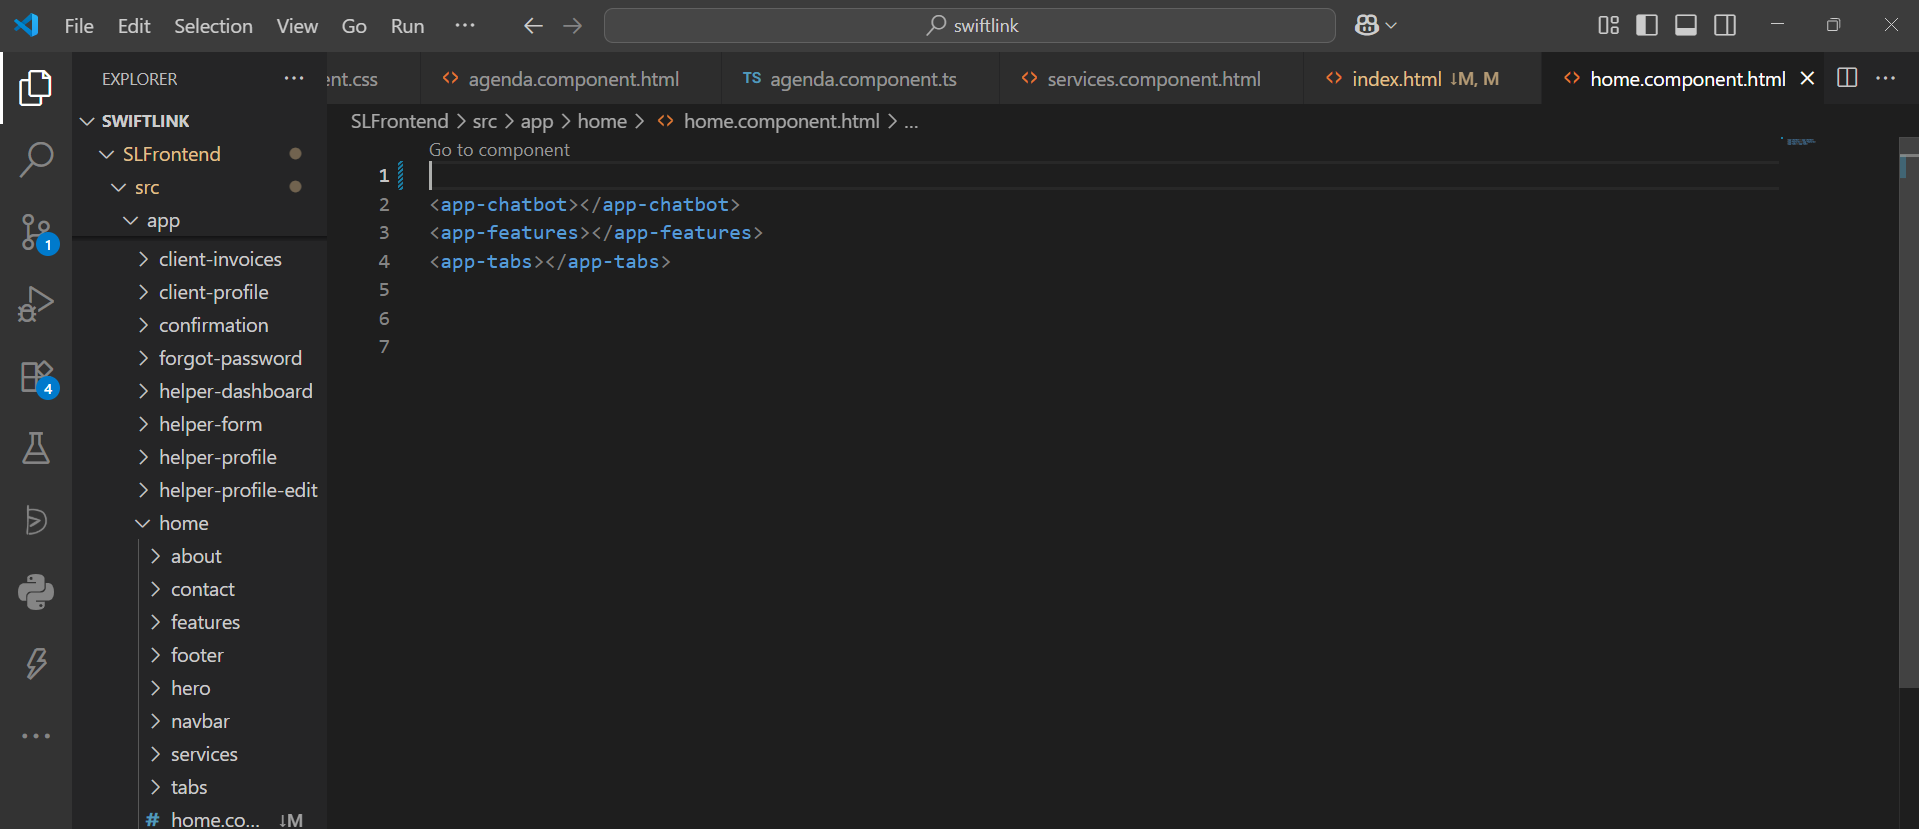
\includegraphics[width=0.9\textwidth]{figures/home comp.png}
    \caption{Structure HTML du composant d’accueil – Angular}
\end{figure}

\noindent
Le fichier \texttt{home.component.html} affiche les éléments de la page d’accueil. Il assemble plusieurs composants personnalisés :
\begin{itemize}
    \item \texttt{<app-chatbot>} : intégration du chatbot interactif.
    \item \texttt{<app-features>} : présentation des avantages de la plateforme.
    \item \texttt{<app-tabs>} : navigation par onglets pour les sections du site.
\end{itemize}

\vspace{0.5cm}

\begin{figure}[H]
    \centering
    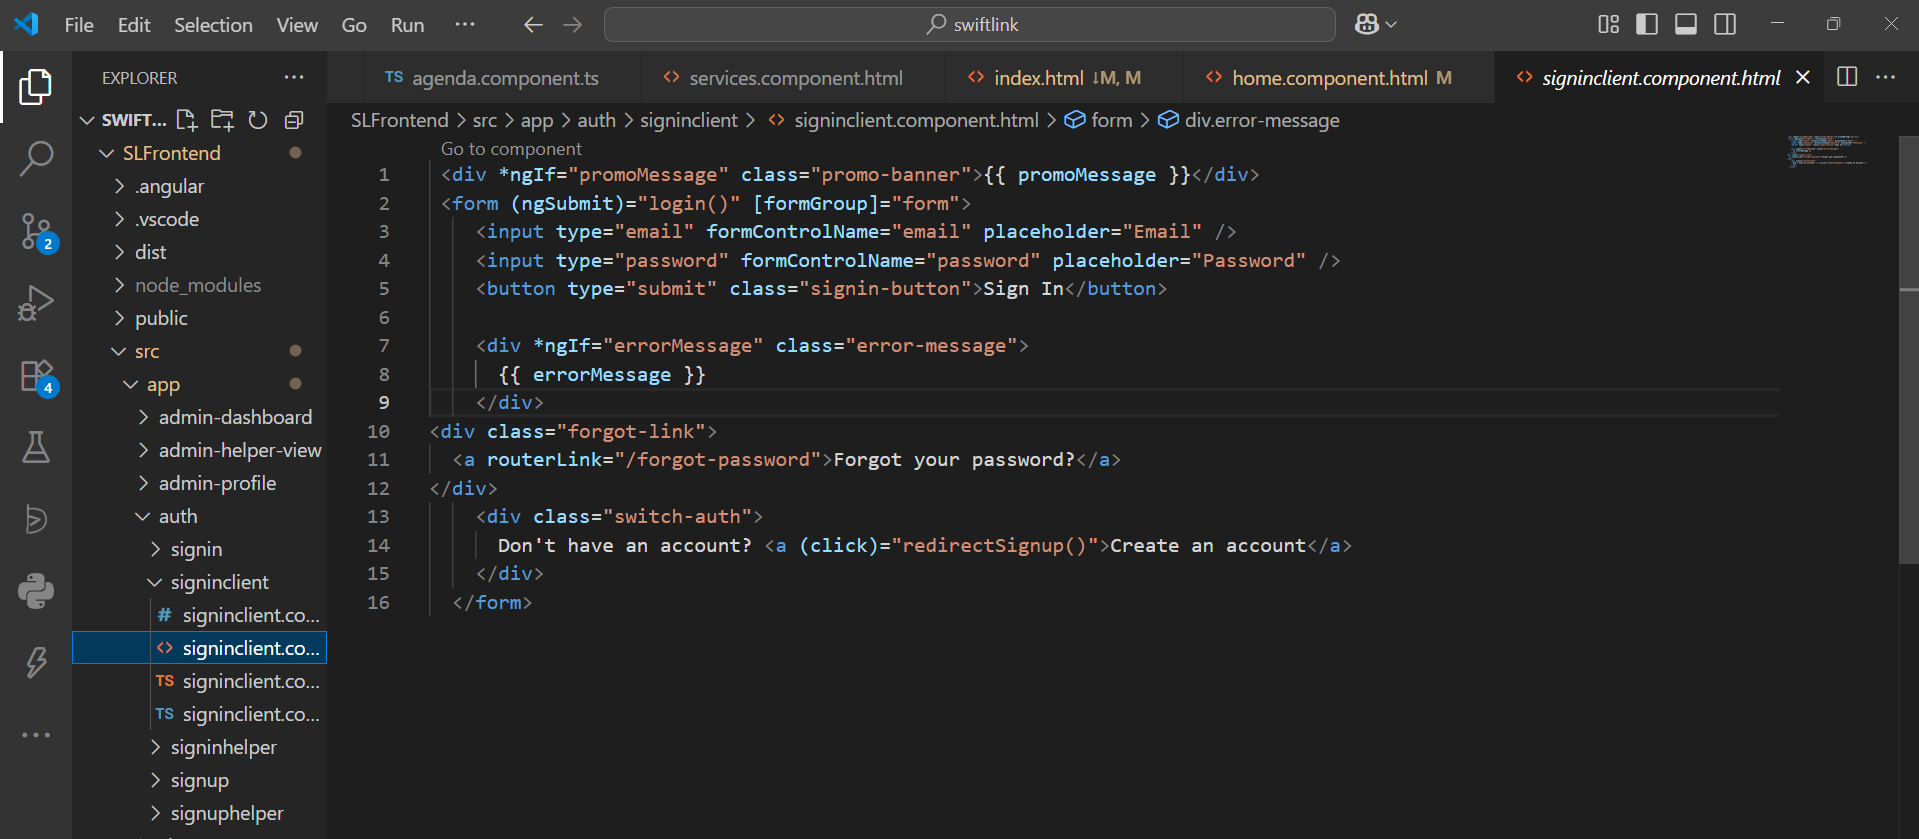
\includegraphics[width=0.9\textwidth]{figures/main.png}
    \caption{Composant HTML de connexion client – Angular}
\end{figure}

\noindent
Le fichier \texttt{signinclient.component.html} permet de construire le formulaire de connexion du client. Il contient :
\begin{itemize}
    \item Un champ email et mot de passe avec liaison au formulaire réactif Angular.
    \item Un message d’erreur dynamique si l’authentification échoue.
    \item Un lien de redirection vers la page d’inscription ou récupération de mot de passe.
\end{itemize}
\section*{Conclusion}

Le Sprint 01 a permis de poser les bases fonctionnelles et techniques du module de gestion des clients. À travers une structuration claire des modèles de données, l’implémentation d’interfaces conviviales et l’intégration réussie du backend et du frontend via une API REST sécurisée, ce sprint marque une avancée significative dans la mise en place de l’infrastructure utilisateur de la plateforme.

Les fonctionnalités développées offrent désormais aux clients la possibilité de créer, modifier et consulter leur profil, tout en assurant une gestion cohérente des informations côté administration. Les choix technologiques retenus, tels que l’utilisation d’Angular pour l’interface et Django REST Framework pour le backend, se sont avérés pertinents et adaptés aux besoins du projet.

Les acquis de ce sprint serviront de socle aux prochains modules à venir (gestion des prestataires, ordres de mission, facturation, etc.) en garantissant une cohérence d’architecture et une réutilisabilité du code.



